\documentclass[11pt]{report}
\usepackage{graphicx}
\usepackage{hyperref}
\usepackage{url}
\usepackage{epstopdf}
\usepackage{listings}
\usepackage{color}
\usepackage{ulem}
\usepackage{float}

\renewcommand\bibname{References}

% reference commands
\newcommand{\fig}[1]{Figure ~\ref{fig:#1}}
\newcommand{\tab}[1]{Table ~\ref{tab:#1}}
\newcommand{\sect}[1]{Section ~\ref{sec:#1}}

\setcounter{secnumdepth}{3}
\setcounter{tocdepth}{3}
\parindent 0pt
\parskip 8pt

%Gummi|061|=)
\title{Project CS 2012 Product Report\\Uppsala University\\}

\author{Daniele Bacarella\\
		Jon Borglund\\
		Paolo Boschini\\
		Kiril Goguev\\
		Faroogh Hassan\\
		Marcus Ihlar\\
		Alexander Lindholm\\
		Knut Lorenzen\\
		Harold Mart\'{i}nez\\
		Thomas Nordstr\"om\\
		Thiago Costa Porto\\
		Linus Sunde\\
		Kim-Anh Tran
}

\date{}
\begin{document}

\maketitle

\begin{abstract}
In Information Centric Networking (ICN), content is delivered to users based on
the name of the requested resource without taking its physical location into consideration.
Based on the NetInf protocol, an Android application backed by an Erlang implementation of a
Name Resolution Service was implemented and both products are presented in this report.
By communicating with each other, the systems store, share and retrieve data objects in an ICN fashion.
In situations of network congestion content is difficult or impossible to retrieve.
Using ICN, the system can provide alternate transfer methods to facilitate the delivering of content.
\end{abstract}

\section{Glossary}
\textbf{API} - Application Programming Interface\\
\textbf{CH} - Content Handler\\
\textbf{CL} - Convergence Layer\\
\textbf{ERNI} - Erlang NetInf\\
\textbf{EH} - Event Handler\\
\textbf{HTML} - HyperText Markup Language\\
\textbf{HTTP} - HyperText Transfer Protocol\\
\textbf{ICN} - Information-centric Networking\\
\textbf{IO} - Information Object\\
\textbf{IDE} - Integrated Development Environment\\
\textbf{JSON} - JavaScript Object Notation\\
\textbf{LRS} - Local Resolution Service\\
\textbf{MAC} - Media Access Control\\
\textbf{MH} - Message Handler\\
\textbf{NDO} - Named Data Object\\
\textbf{NRS} - Name Resolution Service\\
\textbf{NetInf} - Network of Information\\
\textbf{OTP} - Open Telecom Platform\\
\textbf{SAIL} - Scalable and Adaptive Internet soLutions\\
\textbf{SDK} - Software Development Kit\\ 
\textbf{SQL} - Structured Query Language\\
\textbf{TCP/IP} - Transmission Control Protocol/Internet Protocol\\ 
\textbf{UDP} - User Datagram Protocol\\
\textbf{URL} - Uniform Resource Locator\\
\textbf{URI} - Uniform Resource Identifier\\









\tableofcontents

\section{Introduction}
The main purpose of this project was to build an application based on the NetInf protocol. Ericsson Research acted as the customer for this project whereas the IT department of Uppsala university facilitated us with a project room, software and hardware infrastructure.

The project team was divided into two groups where one group was dedicated for developing the front-end of the application whereas the other group was given the task to develop the back-end. The front-end group was called LISA and consisted of five members whereas the back-end group was named ERNI and was made up of eight individuals. The purpose of the application was to use NetInf protocol in an Information Centric Networking (ICN) paradigm to create, share and store Named Data Objects (NDO's). The front-end team developed the user interface of the application using JAVA which the end user could use to perform different operations. The back-end team developed the necessary modules to perform the back-end operations using Erlang/OTP. The details of the functionalities developed by the front-end and back-end teams can be found in the product report. Both teams followed Scrum as the software development methodology.          

This document describes in detail the various tools, methodolgy and equipments we used to achieve our goals. 

\chapter{Preliminaries}
\label{sec:preliminaries}
\subsection{Network of Information}
\subsection{Open Netinf and thesis}

\section{Development Languages}
\subsection{Java-Android}

Since Elephant is being developed for Android it was all but natural to use Java. The fact that both OpenNetInf and a closely related previous master thesis \cite{masterthesis} further solidified this decision. Java is an imperative object-orient programming language.

något om android sdk
\subsection{Erlang}
Erlang is a concurrent, functional, fault-tolerant language with great scalability and ease of distribution. It was developed by Ericsson in the mid 80's and became open source 1998.\cite{otpInAction} These factors among others such as the client being Ericsson Research made Erlang the choice of language for the NRS implementation.
Another reason for choosing Erlang is that it uses the idea of modules and nodes as a primary platform for serving a function, which allowed the product to be broken up into several parts which could be developed concurrently.
\subsection{Javascript}
Javascript was used when the backend group decided to create a simple http interface to the NetInf Name Resolution server in order to show a proof of concept (NetInf streaming). Javascript was used to calculate the hash of files for streaming as well as for asynchronious communication with the NRS.

\chapter{Goals and Scope}
\label{sec:goals}
\section{Frontend}

\subsection{NetInf Enabled Browser}

The goal of the frontend is to produce Elephant, a NetInf enabled browser for Android devices. The browser should utilize NetInf technology to retrieve web page from other nearby devices and/or caching nodes, if possible, in order to reduce the usage of the 3G uplink commonly used to access the Internet on mobile devices. This is done so that congestion in the 3G network can be avoided. The NetInf traffic should conform to the work in progress HTTP convergence layer \cite{netinfproto}. Web pages should be split into several parts to be able to benefit from being available from multiple sources.

To accomplish this we need the possibility to:

\begin{itemize}
	\item Inject existing web pages into the NetInf network as NDOs.
	\item Given a traditional web URL be able to find the corresponding NDO.
	\item Get NDOs from other devices.
\end{itemize}

See Section \ref{sec:Elephant} for details on how this was solved by the Elephant browser.

The following problems was considered to be out of scope:

\begin{itemize}
	\item Privacy
	\item Security
	\item Dynamic Content
	\item Battery Consumption
	\item Bluetooth Congestion
\end{itemize}

Privacy and security are both very important aspects, but would require complex considerations. They are areas that will require future work.

Dynamic content is relevant as it is often changes in content (e.g. newspapers, Facebook, Twitter) that interests users. However this would add a lot of complexity to the problem since dynamic content means the mapping from traditional web URL to NDO would be constantly changing.

Battery consumption was discusses and the simple solution of allowing users to disable battery draining technologies such as Bluetooth was decided upon. Hopefully, the battery problem will be solved by technological advancements.

A final problem that was not taken into consideration was possible congestion in the Bluetooth network because of large amount of devices.
\section{Backend}
In this section we describe the goals and scope set by the backend team for this project.

\subsection{Goals}
The following goals were set for the Erlang implementation of the NRS:
\begin{enumerate}
 \item {Build a Name Resolution Service (NRS) for the Erlang NetInf application.}\\
 \item {Be able to publish, store and retrieve Named Data Objects (NDO's) in a NetInf network.}\\
 \item {Make each NetInf node a caching node that can store NDO's.}\\
 \item {Make the back-end processes distributed, concurrent and fault tolerant.}\\ 
 \item {Be able to stream video using our Erlang NetInf application.}\\
  \end{enumerate}

\subsection{Scope}
The scope of the NRS application is limited to providing all the functionalities outlined in the NetInf Protocol draft document. \cite{netinfproto} This document outlines what information a NetInf Get, Publish and Search message should contain. It also defines how a Get, Publish and Search response message should look like. Apart from that it also covers specifications for the HTTP and UDP convergence layers. We made sure that our application followed all these specifications accurately. Providing video streaming was not part of the scope at the beginning of this project but at the client's request preliminary(proof-of-concept) work was done, however readers should note that the video streaming is not meant to be a complete product and the development team encourages further research into this product.


\chapter{Product Description}
\label{sec:product}

\section {Frontend - Android Client}
The following section will describe the product the front-end team developed during the course.
The product consists of two different applications: Elephant, the web browser, and an implementation
of the NetInf services that support Information-Centric Networking.

\subsection{Elephant Web Browser}
The web browser application is a simple implementation

\subsection{NetInf Service}


\section {Backend}

The customer agreed on having an Erlang NetInf NRS. The backend product implements the, as of writing, current draft of the NetInf Protocol\cite{netinfproto} in a purely functional language. The product promises a high level of scalability and fault-tolerance. The client initially asked for only the NRS as a product however the backend team was able to complete the initial product in a timely manner, allowing for applications of this network technology to be explored. 


\subsection {Erlang NetInf Name Resolution Service}
The first of the two deliverables from the backend team to the customer. The Erlang NetInf NRS provides a new way to organize and retrieve data on the Internet. Based on an initial NetInf NRS protocol draft from development teams such as SAIL and Ericsson Research\cite{netinfproto}. This product allows for flexibility and extension of the existing protocol.

Erlang's concept of modularization allowed the team to break up the NRS functionality into distinctive convergence layers, runtime database switching, and even allow for a proof-of-concept data streaming client/protocol. 

\subsection{NetInf Video Streaming Client/Protocol}

The last of the deliverables from the backend team. The customer requested a proof-of-concept video streaming protocol and HTML client interface which lies on top of the Erlang NetInf NRS technology. The streaming protocol is a completely new addition to the NetInf draft\cite{netinfproto}. The team developed a way to utilize the code and transporting mechanism of the first product in order to stream video content. Along with the protocol outlined in Appendix C \ref{VideoDraft}, the team has created a HTTP interface client which allows the user to see the streaming protocol in action in addition to accessing the NRS functionality. This particular product was not specified in the initial conversations with the customer in September, but was added late in the development cycle and is a proof-of-concept.

\subsubsection{First Implementation}
In addition to normal NRS functionality, a HTTP transfer-dispatcher had to be implemented in order to transfer of chunks between clients. The streaming works by clients subscribing to a stream from a specific NRS. Once connected the client, with a constant interval will ask the NRS where to find these chunks. All the chunks are transferred via the transfer-dispatcher.
The playback of the video chunks is done by polling the local NRS, this implies that every client has its own NetInf node running. See figure \ref{fig:stream-seqorgmod}. The benefit of using this approach is that only one NDO containing the filename has to be published. The receiver can then derive the chunks locations, by appending the chunk number to the end of the locators provided in the filename NDO.

\begin{figure}[h!]
	\centering
		\includegraphics[width=0.75\textwidth]{./img/sequence_diagram_streaming_orgmod.png}
    	\caption{Original/Modified Chunked Data Transfer}
	\label{fig:stream-seqorgmod}
\end{figure}

\subsubsection{Modified NetInf Streaming}
Due to a request from the customer a more true NetInf implementation of streaming was implemented. Instead of using the transfer-dispatcher between the client nodes a workaround was added that disabled content validation, this resulted in fetching of chunks via NetInf messages. The polling logic is still the same as first implementation, seen in figure \ref{fig:stream-seqorgmod}. Instead of using ordinary HTTP locators, the receiver is required to modify the \textit{NetInf GET requests} to get the chunks. This is done by replacing the hash algorithm with the custom hash name \textit{demo}. For example to get the first chunk of \textit{ni:///sha-256;abc}, the request should contain \textit{ni:///demo;abc1}. The HTTP transfer-dispatcher is still used to transfer the chunks to the HTML-interface.

\subsubsection{Pure NetInf Streaming}
To be able to evaluate the modified NetInf streaming another implementation was added. This implementation uses NetInf searches and gets for chunks. See Figure~\ref{fig:stream-seq-pure}. In this implementation the stream source is required to publish each chunk to the NRS, and modify the NDO metadata with the stream name and stream chunk number. The receiver is then required to search for each chunk to find it. 

\begin{figure}[h!]
	\centering
		\includegraphics[width=0.75\textwidth]{./img/sequence_diagram_pure_streaming.png}
    	\caption{Chunked Data Transfer With Pure NetInf}
	\label{fig:stream-seq-pure}
\end{figure}

\subsubsection{Streaming Frontend}
To merge the chunks, a simple HTML5 frontend was created. HTML was chosen to make the player platform independent.
In both implementations the player starts a JavaScript that continuously polls the local NetInf node for the chunks through the HTTP dispatcher.
The difference is that the pure NetInf player uses the NRS search to build the playlist, while the modified NetInf version only increases the chunk number.


\chapter{System Architecture}
\label{sec:architecture}
\section{Architecture Overview}
The system is a combination of frontend and backend subsystems that communicate using network protocols including HTTP and Bluetooth. Figure~\ref{fig:overall_arch} shows how messages can flow between the different subsystems. All messages are of a request-response type, therefore messages are always flowing in both directions between subsystems. The messages contain NetInf get, publish or search requests except for messages emitted from the Elephant web browser to the Internet, these are normal HTTP requests. 

The following sections describe the different subsystems in detail.
\begin{figure}[H]
	\centering
\centerline{\includegraphics[width=1.2\textwidth]{./img/overall_arch.png}}
\caption{The Elephant browser initially requests an object from the NetInf service, if the object is not found the request will be forwarded to an Erlang NRS. The Erlang NRS responds with object or locators to the objects if the object is present in the NetInf network. If the object is not found within the NetInf network, the Elephant browser will try to fetch it from the Internet and then publish it to the NetInf Service which in turn will send a publish request to the NRS.}
\label{fig:overall_arch}
\end{figure}
\definecolor{javared}{rgb}{0.6,0,0} % for strings
\definecolor{javagreen}{rgb}{0.25,0.5,0.35} % comments
\definecolor{javapurple}{rgb}{0.5,0,0.35} % keywords
\definecolor{javadocblue}{rgb}{0.25,0.35,0.75} % javadoc

\lstnewenvironment{code}[1][]%
	{\minipage{\linewidth} 
		\lstset{language=Java,
			basicstyle=\ttfamily,
			keywordstyle=\color{javapurple}\bfseries,
			stringstyle=\color{javared},
			commentstyle=\color{javagreen},
			morecomment=[s][\color{javadocblue}]{/**}{*/},
			numbers=left,
			numberstyle=\tiny\color{black},
			stepnumber=1,
			numbersep=10pt,
			tabsize=4,
			showspaces=false,
			showstringspaces=false}}
	{\endminipage}

\section{NetInfService}
\label{sec:NetInfService}

NetInfService is the first of two Android applications. It provides a NetInf node which can be accessed through a RESTful API. This allows any application running on the same device as the NetInfService to access NetInf functionality through simple HTTP requests. The interface is described in detail in Section \ref{sec:RESTful API}. NetInfService is based on the work done in a previous master thesis \cite{hugomiguel} and uses and extends OpenNetInf to provide this functionality. An overview of the design of NetInfService can be seen in Figure \ref{fig:netinfserviceoverview}, the individual components are described below. 

\begin{figure}
	\centering
		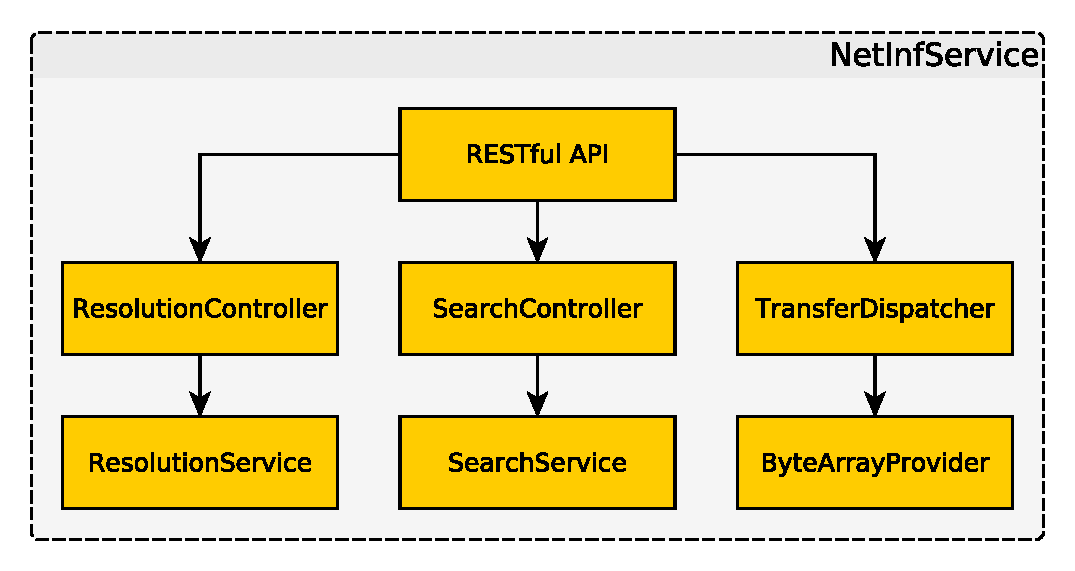
\includegraphics[width=0.75\textwidth]{./img/netinfservice}
    	\caption{NetInfService Overview}
	\label{fig:netinfserviceoverview}
\end{figure}

Figure \ref{fig:netinf-controlflow} shows a picture of the internal control flow of the NetInfService,
and provides the packages and/or source files, as well as some text and arrows describing the control flow.
The digits on the connections between boxes illustrate the order actions are taken.


\begin{figure}
\centering
\centerline{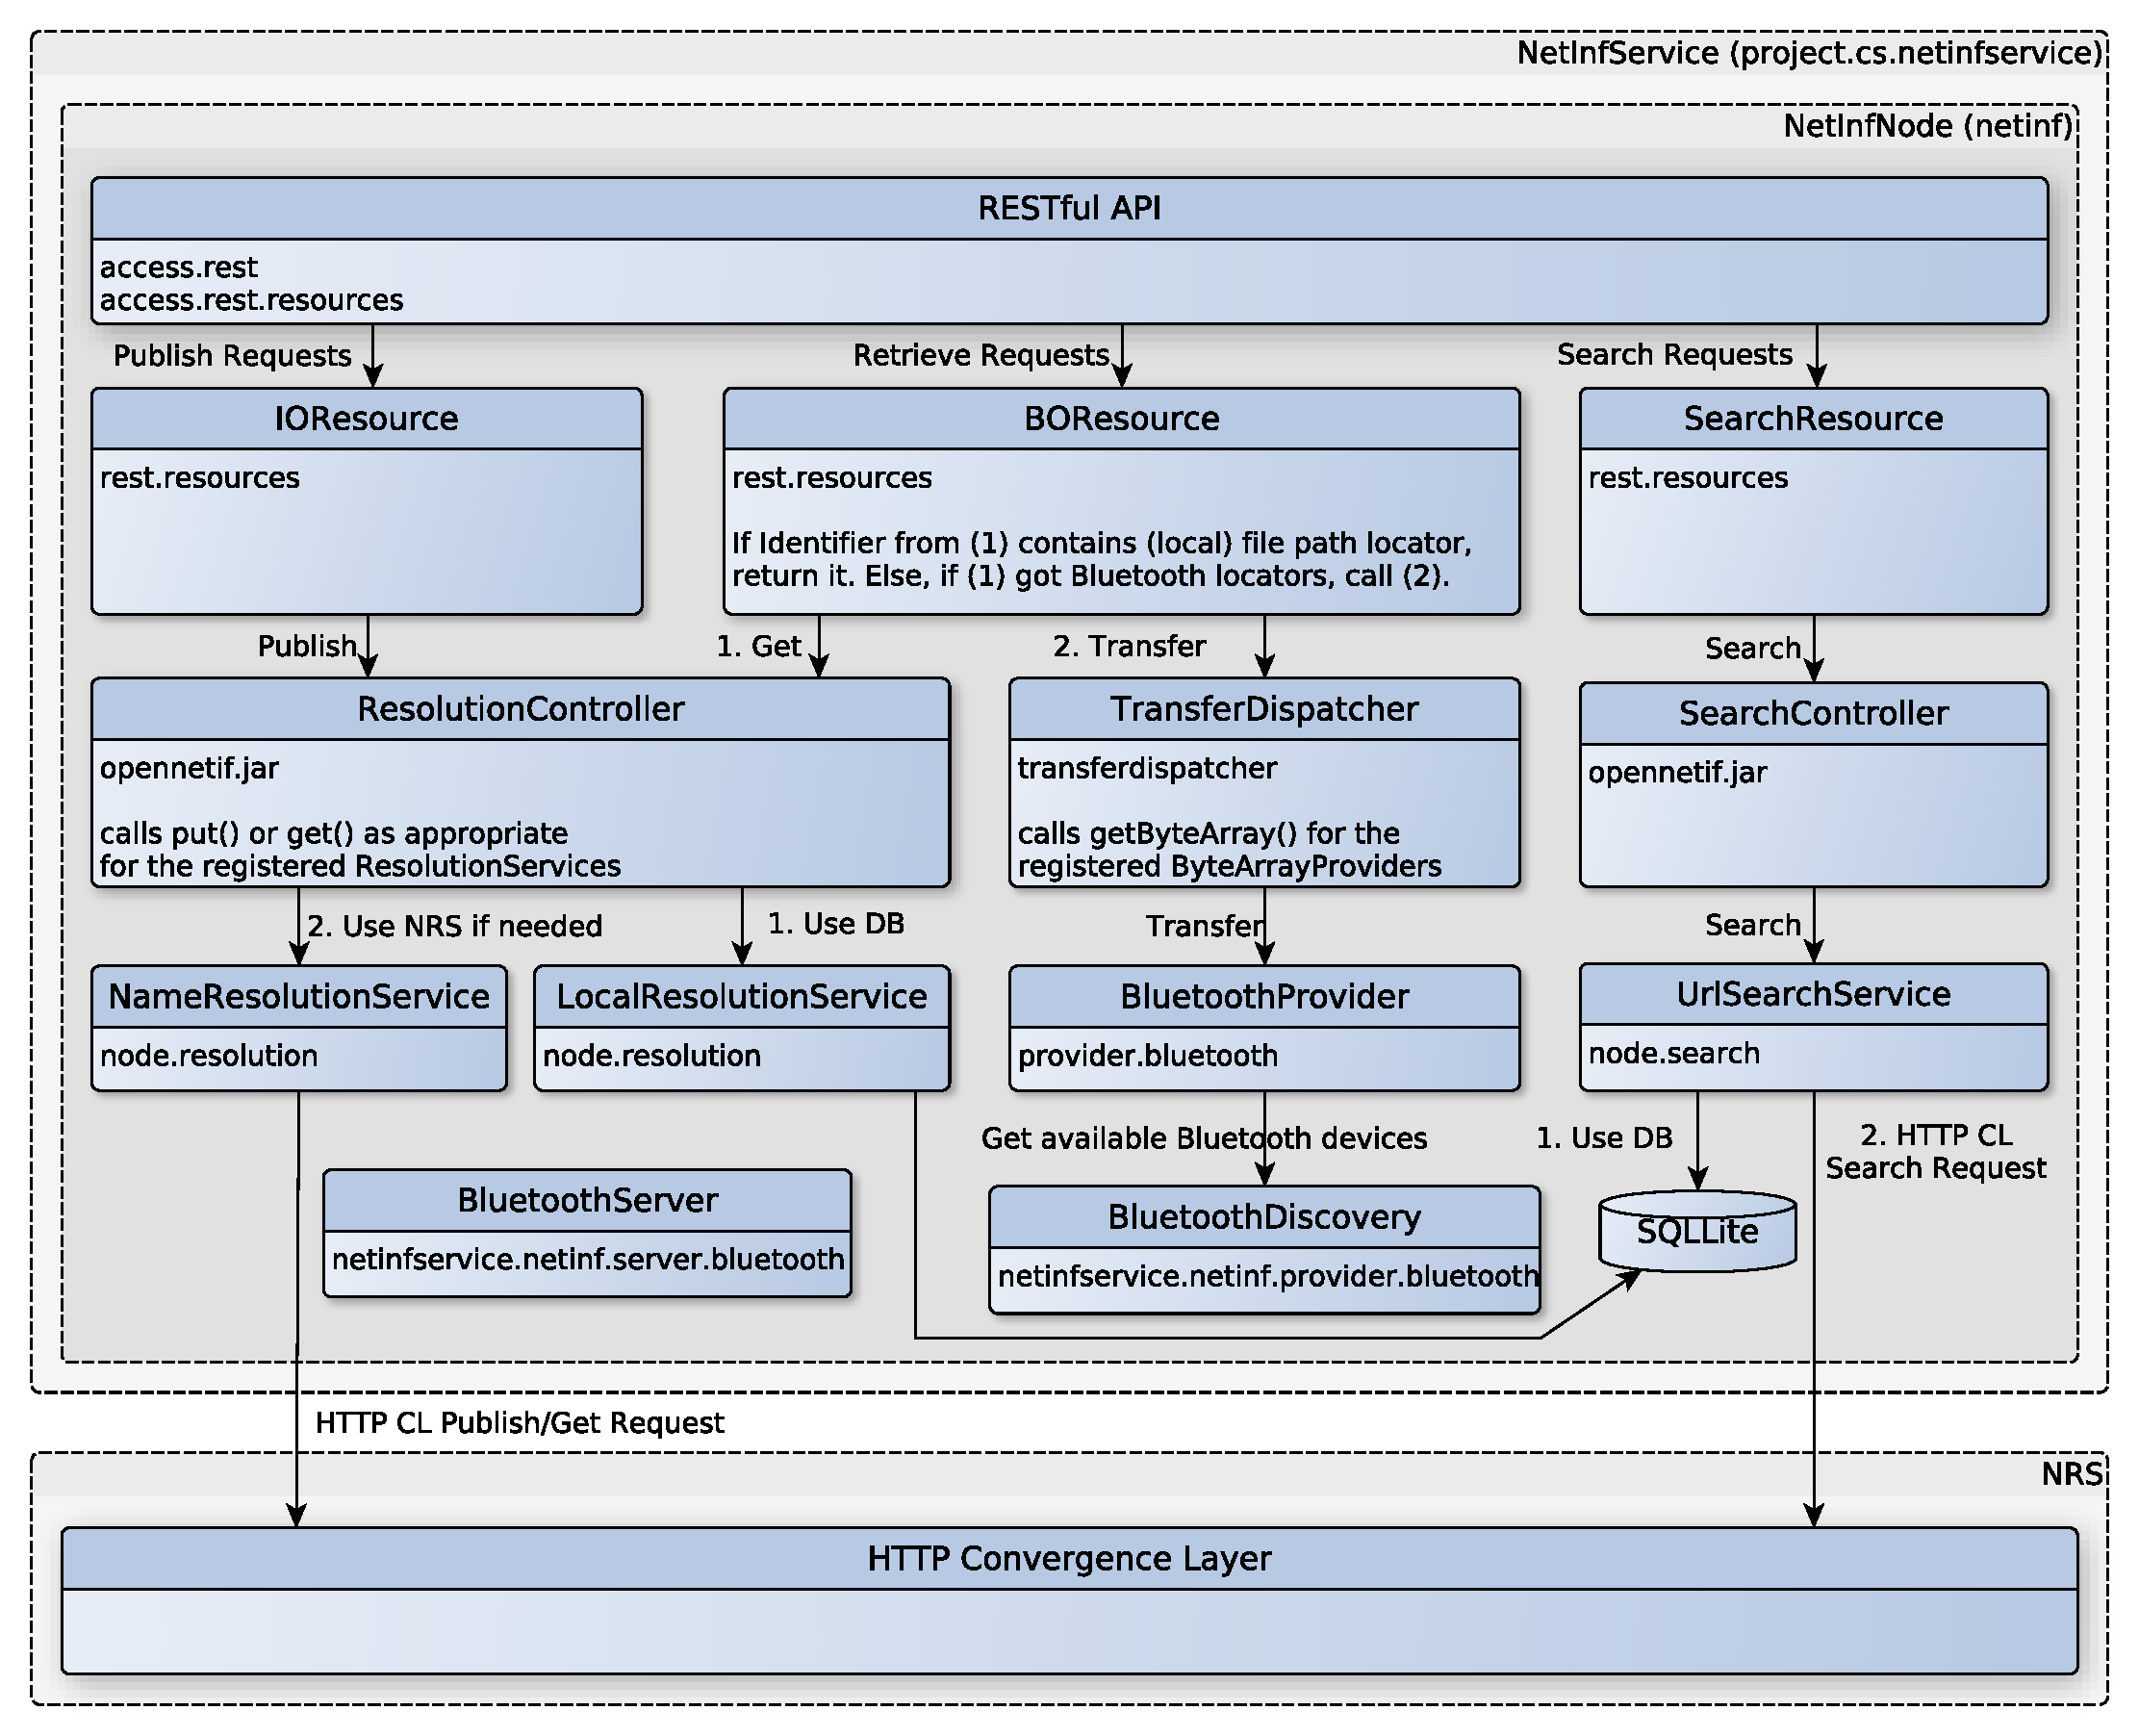
\includegraphics[width=1.4\textwidth]{./img/flowchart-NetInf.pdf}}
\caption{NetInfService Control Flow}
\label{fig:netinf-controlflow}
\end{figure}

\subsection{Configuration}
\label{sec:Configuration}

The default settings for NetInfService are stored in the properties file "assets/config.properties". This includes but is not limited to NRS IP address, NRS port and RESTful API port. Some of these settings can be changed when running the NetInfService on an Android device. This does not change the default values in the properties file but the changes are instead stored using the default Android shared preferences file, which is persistent.

\subsection{RESTful API}
\label{sec:RESTful API}

The RESTful API receives HTTP requests for NetInf functionality. Depending on the type of request, the ResolutionController, SearchController or TransferDispatcher is called. Publish requests are handled by the ResolutionController. Retrieve requests first trigger a get request using the ResolutionController and then, if the get response contained locators, transfer the file using the TransferDispatcher. Search requests are handled by the SearchController.

The HTTP request uses the following format:

\begin{center}
http://\{Host\}:\{Port\}/\{Prefix\}?\{key1\}=\{value1\}\&\{key2\}=\{value2\}...
\end{center}

Since the NetInfService should be running on the same device as the application that is using it, the host would most likely be either localhost or 127.0.0.1. The default port is 8080, for changing these settings see Section \ref{sec:Configuration}. The key-value pairs must be URL encoded as they can contain illegal characters.

\subsubsection{Publish}

Publish request uses the prefix \emph{publish}.

It requires the following key-value pairs:

\begin{tabular}{ | l | l | }
	\hline
	key & value  \\ \hline \hline
	hash & The hash of the object being published.  \\ \hline
	hashAlg & The hash algorithm used to hash the object. \\ \hline
	ct & The MIME content-type of the object being published. \\ \hline
\end{tabular}

The following key-value pairs are optional:

\begin{tabular}{ | l | l | }
	\hline
	key & value  \\ \hline \hline
	btmac & The Bluetooth MAC address of the publishing device. \\ \hline
	meta & Metadata as a JSON string. \\ \hline
	filepath & Path to the file being publish. \\ \hline
\end{tabular}

\begin{itemize}
	\item btmac: The Bluetooth MAC address of the publishing device, it will be added as a locator to the published object.
	\item meta: The metadata \cite{netinfproto} of the object that is being published. Remember to URL encode illegal characters.
	\item filepath: The file path of the object that is being published. If this is present, a full put is done, otherwise not.
 \end{itemize}

A successful publish returns HTTP status code 200. Any other code indicates that something went wrong and should give an indication of what went wrong.

Below is an example of how a HTTP publish request could look like, notice the URL encoding:

http://localhost:8080/publish?hash=TcoP1fQkoxsDq4B8uud\%2Bsyvy0Inu0c7hVLOv7UWN4Nw \\ \&hashAlg=sha-256\&ct=text\%2Fplain\&btmac=F0\%3AE7\%3A7E\%3A3F\%3AD2\%3A43

Unencoded it would look like:

http://localhost:8080/publish?hash=TcoP1fQkoxsDq4B8uud+syvy0Inu0c7hVLOv7UWN4Nw \\ \&hashAlg=sha-256\&ct=text/plain\&btmac=F0:E7:7E:3F:D2:43

\subsection{Retrieve}

Retrieve requests use the prefix \emph{retrieve}.

It requires the following key-value pairs:

\begin{tabular}{ | l | l | }
	\hline
	key & value  \\ \hline \hline
	hash & The hash of the object being published.  \\ \hline
	hashAlg & The hash algorithm used to hash the object. \\ \hline
\end{tabular}

A successful retrieve returns HTTP status code 200. The HTTP response should contain a JSON object with two key-value pairs. The key \emph{path} should contain a local file path to the retrieved object. The key \emph{ct} should contain the MIME content-type of the retrieved object. Any other code indicates that something went wrong and should give an indication of what went wrong.

Below is an example of how a HTTP retrieve request could look like, notice the URL encoding:

http://localhost:8080/retrieve?hash=TcoP1fQkoxsDq4B8uud\%2Bsyvy0Inu0c7hVLOv7UWN4Nw \\ \&hashAlg=sha-256

Unencoded it would look like:

http://localhost:8080/retrieve?hash=TcoP1fQkoxsDq4B8uud+syvy0Inu0c7hVLOv7UWN4Nw \\ \&hashAlg=sha-256

\subsection{Search}

Search requests use the prefix \emph{search}.

It requires the following key-value pairs:

\begin{tabular}{ | l | l | }
	\hline
	key & value  \\ \hline \hline
	tokens & The tokens being searched for.  \\ \hline
\end{tabular}

The following key-value pair is optional:

\begin{tabular}{ | l | l | }
	\hline
	key & value  \\ \hline \hline
	ext & An optional JSON, meant for future extensions. \\ \hline
\end{tabular}

\begin{itemize}
	\item tokens: Currently NetInfService only supports one token. This should be changed to accept a string of space separated search tokens to follow specification.
	\item ext: The ext field is meant for future extensions. It is allowed, but currently ignored.
 \end{itemize}

Below is an example of how a HTTP search request could look like, notice the URL encoding:

http://localhost:8080/search?tokens=http\%3A\%2F\%2Fwww.ericsson.com\%2F

Unencoded it would look like:

http://localhost:8080/search?tokens=http://www.ericsson.com/

\subsection{ResolutionController}
\label{sec:ResolutionController}

The ResolutionController handles a number of ResolutionServices. Each ResolutionService should provide publish, get, and delete functionality using some convergence layer or equivalent. Currently there are two ResolutionServices, the LocalResolutionService which uses a local SQLite database and the NameResolutionService which communicates with a specific NRS using the HTTP convergence layer.

\subsubsection{NameResolutionService}

The NameResolutionService uses the Named Information URI \cite{ninames} and the HTTP convergence layer \cite{netinfproto} to communicate with a single NRS. Currently the NameResolutionService supports publish and get. Delete is not yet supported but the framework for its implementation is there.

\subsubsection{LocalResolutionService}

The LocalResolutionService uses a connection to the device's local SQLite database. The LocalResolutionService has higher priority than the NameResolutionService meaning that when preforming a get request the LocalResolutionService will be used first and then if needed the NameResolutionService as well.

\subsection{SearchController}
\label{sec:SearchController}

The SearchController handles a number of SearchServices. Each SearchService should provide search functionality 
using some convergence layer or equivalent. Currently there is one SearchService, the UrlSearchService, 
which provides search functionality using a single token which is assumed to be a URL.

\subsubsection{UrlSearchService}

The UrlSearchService provides the functionality to search for a single token in the local database 
used by the LocalResolutionService and then, if not found, using the HTTP convergence layer to search 
in the NRS used by the NameResolutionService.

\subsection{TransferDispatcher}
\label{sec:TransferDispatcher}

The TransferDispatcher handles a number of ByteArrayProviders. Each ByteArrayProvider should provide functionality to retrieve a file (as a byte array) in some way. Currently there is one ByteArrayProvider, the BluetoothProvider, which uses Bluetooth to transfer files between Bluetooth enabled devices.

\subsubsection{BluetoothProvider}
\label{sec:BluetoothProvider}
The BluetoothProvider provides the functionality to retrieve the bytes of an NDO through a specified Bluetooth locator. It first tries to establish a connection to the remote
Bluetooth device. If successful, it requests the bytes of an object by sending the hash value
that describes the object. As a response, the provider retrieves the bytes of the object, if
it was available on the remote Bluetooth device.

\subsubsection{BluetoothServer}
The BluetoothServer continuously listens to incoming Bluetooth file requests. 
If a remote device wants to connect to the local device, the BluetoothServer establishes
a BluetoothSocket through which both devices can communicate with each other.
The BluetoothServer expects to receive a string that represents the hash
of a requested object. Using this hash, the BluetoothServer will send back
the byte arrays of the corresponding object, if available. 

\section{Elephant}
\label{sec:Elephant}

Elephant is the second Android application. It is a simple browser which uses NetInf through the NetInfService to cache and share web pages.

The idea behind the Elephant browser is simple. When a traditional web URL is entered into the address bar and the refresh button is clicked, instead of downloading the web page from the Internet the browser first tries to use NetInf to retrieve the web page.

This is done by using the NetInfService. For the entered URL and each resource it links to:
\begin{enumerate}
	\item Search for the hash of the URL/resource.
	\item Get the file with the given hash.
	\item Possibly publish the file so that other devices can retrieve the file from this device.
\end{enumerate}

If the search or get fails for any reason, be it a timeout, no matches found or something else, the webpage is downloaded using the a standard HTTP request.

\subsection{Configuration}
\label{sec:ConfigurationElephant}

The default settings for Elephant are stored in the properties file "assets/config.properties". This includes but is not limited to RESTful API IP address, RESTful API port and RESTful API timeouts.

\subsection{Control Flow}
\label{sec:Control Flow}

Figure \ref{fig:macro-controlflow} shows an overview of the control flow of the interaction between Elephant and NetInfService.
Figure \ref{fig:application-controlflow} shows a picture of the internal control flow of the Elephant web browser, providing the packages and/or source files that are
involved in different parts of the program, as well as some text and arrows describing the control flow.

The NetInfService mainly does its work by passing around Identifiers and NDOs (each encapsulating an Identifier).

An Identifier contains information about an NDO. The most important pieces of information in these applications are:
\begin{itemize}
\item Hash Algorithm
\item Hash
\item Content-Type
\item Metadata (as a JSON string)
\end{itemize}

NDOs can contain attributes. In these applications the only used attributes are locator attributes. More specifically locators pointing to other Bluetooth devices and locators pointing to the local file system.

\begin{figure}
\centering
\centerline{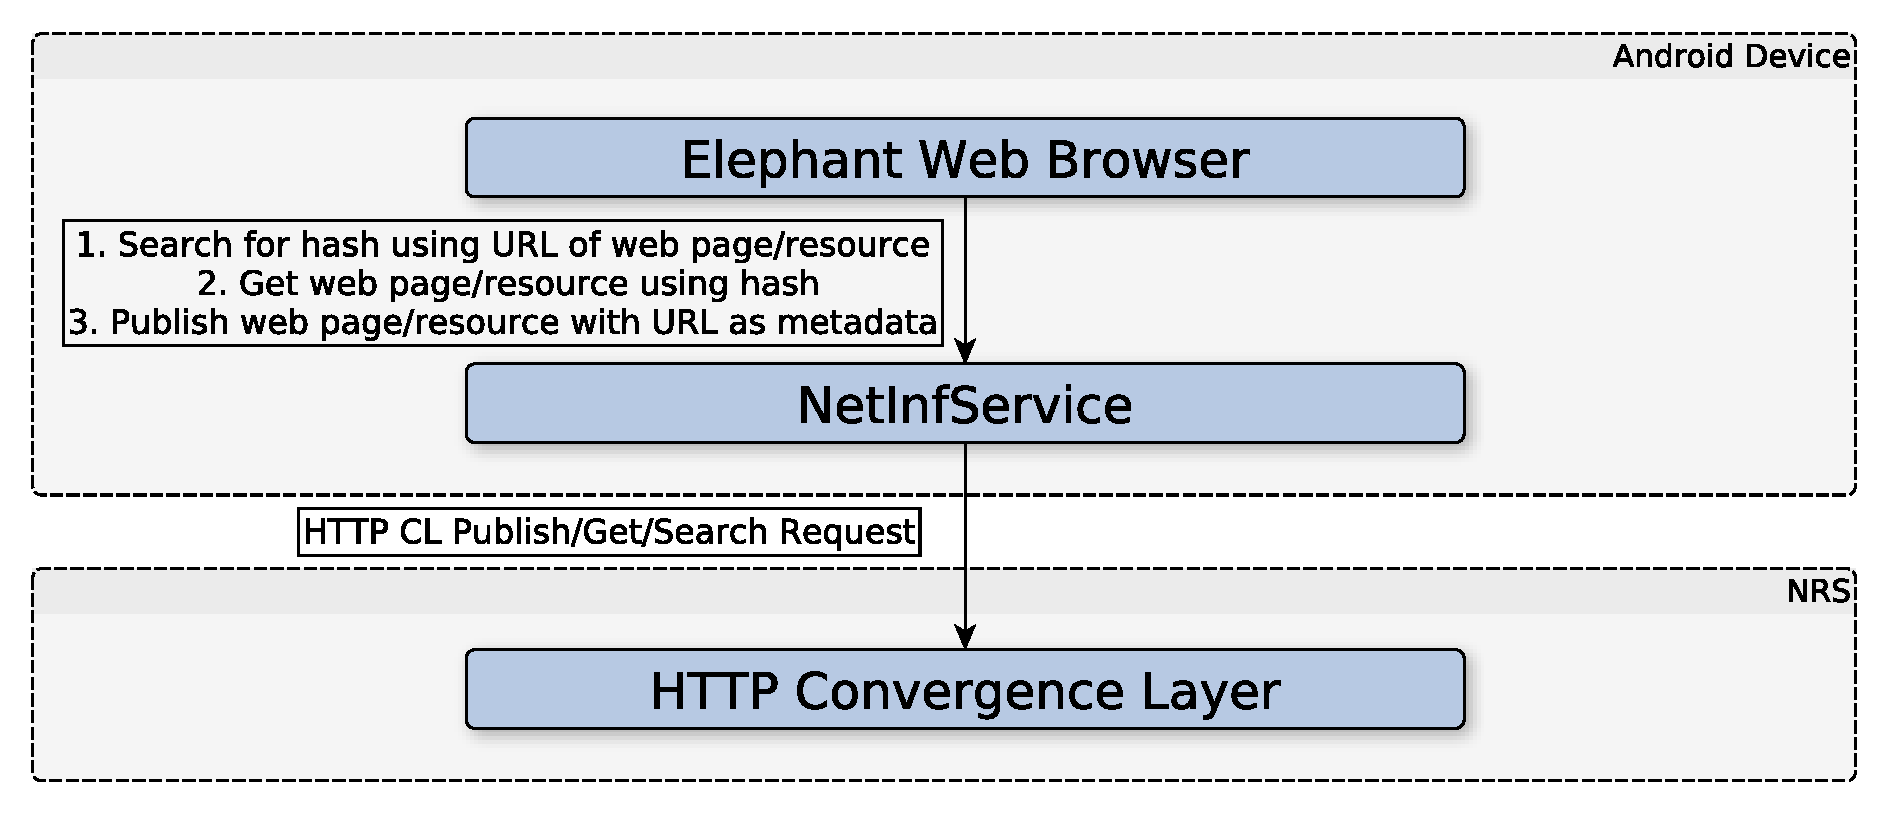
\includegraphics[width=1.4\textwidth]{./img/flowchart-macros.pdf}}
\caption{Elephant/NetInfService Control Flow}
\label{fig:macro-controlflow}
\end{figure}

\begin{figure}
\centering
\centerline{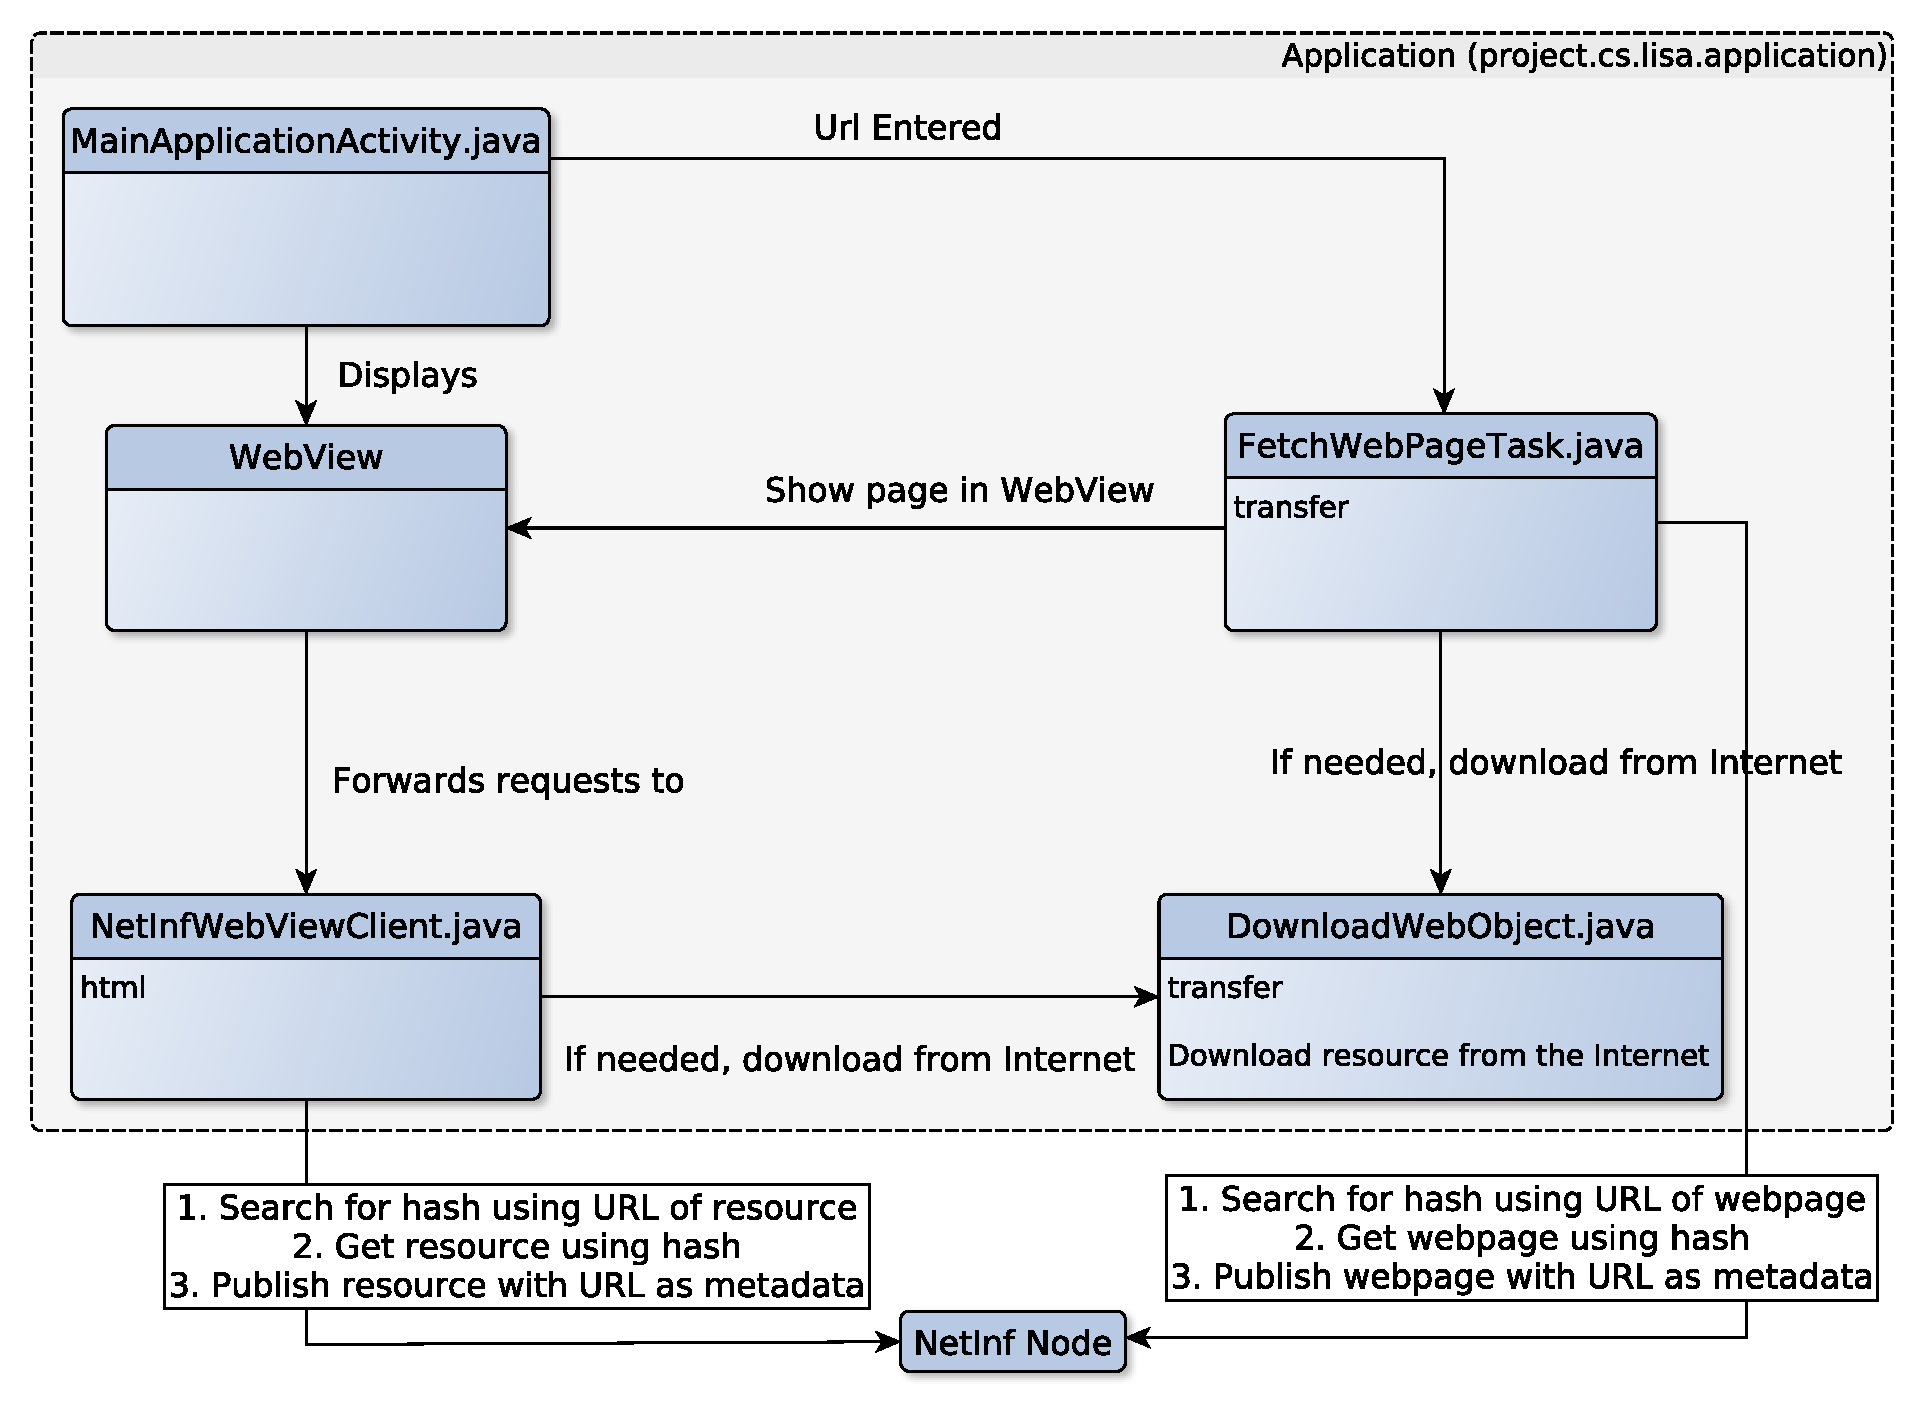
\includegraphics[width=1.4\textwidth]{./img/flowchart-application.pdf}}
\caption{Elephant Control Flow}
\label{fig:application-controlflow}
\end{figure}

\subsection{RESTful API Access}

Access to the RESTful API is handled by the subclasses of NetInfRequest. There are three subclasses NetInfPublish, NetInfRetrieve and NetInfSearch corresponding to the API calls for publish, retrieve and search. NetInfRequest extends the class AsyncTask provided by Android, and hence all subclasses of NetInfRequest are also AsyncTasks.

These classes can be used in two ways. Either by doing a blocking call:

\begin{code}[language=Java]
	// Create a new search
	NetInfSearch search = new NetInfSearch("tokens", "ext");
	// Execute the search
	search.execute();
	// Block until the search response is available
	NetInfSearchResponse searchResponse =
	        (NetInfSearchResponse) search.get();
	// Do things with the response...
\end{code}

Or in a non-blocking way by overriding the function that is called when the response becomes available:

\begin{code}[language=Java]
	// Create a new search
	NetInfSearch search = new NetInfSearch("tokens", "ext") {
            @Override
            public void onPostExecute(NetInfResponse response) {
                NetInfSearchResponse searchResponse =
                        (NetInfSearchResponse) response;
				// Do things with the response...
            }
    }
    // Execute the search
	search.execute();
\end{code}


\section {Erlang NetInf NRS}

\section {Overall design}

The architecture of the entire system consists of different processes and modules which interact with each other. There are two distinct process types: persistent and non-persistent. The persistent processes will run for the entire uptime of the system whereas the lifetime of a non-persistent process is the duration of its given task. Figure x below shows the current system design.

\begin{figure}[h!]
	\centering
\includegraphics[scale=0.6]{./img/process_hierarchy.png}
\caption{Current system design}
\end{figure}

\subsection{Architecture layers}

The system architecture is divided into four distinct layers a network layer (http, udp) convergence layer, an internal Erlang NetInf layer and a storage layer. Within these layers lie the modules(Erlang processes) which are responsible for specific functions such as sending/receiving convergence layer messages, sanitizing messages, forwarding, accessing databases/file systems and logging.

\subsection{NetInf Messaging}

According to the draft specification(see appendix D-draft) NetInf has three well defined messages which comprise of the core functionality of the system. The following sections describe the purpose and flow of each of these messages.

\subsubsection{Named Data Objects}
In addition to the messaging component, NetInf describes any piece of information as a Named Data Object(NDO). In the current state of networks, the same piece of information is considered to be location based and mutable with many copies of the same information lying around. The purpose of an NDO is to provide a convenient way for the protocol to be able to catalogue and preform operations such as storing, retrieving and finally searching for information and eliminating need for location based information.


\subsubsection{Publish}

NetInf describes a Publish message which consists of the following fields:

\begin{description}
\item[URI]  - Contains the hash of the NDO. It is unique to the peice of information that is going to be published into the system. It is also mandatory.
\item[msgid] - A mandatory field as well and it is a unique number(integer). 
\item[loc1] - An optional field, this is the I.P address of the device that created the information that will be shared.
\item[loc2] - Same as the above.
\item[ext] - An extension field, it is responsible for containing the meta data in JSON format.
\item[rform] - 
\item[fullPut]
\end{description}

\subsubsection{Get}

NetInf describes a Get message which consists of the following fields:

\begin{description}
\item[URI]
\item[msgid]
\item[loc1]
\item[loc2]
\item[ext]
\end{description}


\subsubsection{Search}

NetInf describes a Search message which consists of the following fields:

\begin{description}
\item[msgid]
\item[tokens]
\item[rform]
\item[ext]
\end{description}



\newpage
\subsection {Dependencies}

The system architecture for the backend relies on a few external libraries. The following are important for the system to run well. 

\begin {enumerate}
\item Erlang Cowboy - with it's own set of dependencies Ranch, and Crypto
\item Erlang RTS 
\item Erlang covertool
\item Erlang JSON library
\item Riak - with search hooks and a Key-Value(KV) bucket installed.
		(Only used for using the system with Riak database)
\end {enumerate}


\subsection {Configurations}

Since the system is supposed to be modular, configuration files are also implemented. 

Configuration files allow the user of the system to quickly start it with a predetermined setup, things such as which database to use, which convergence layers are supported, and timers for various functionality are also stored here for quick use and editing. The benifit of using erlang specific configuration files is the great way they are organized, giving a highly readable and easy to swap out functionality. 

We have created 2 config files which live in the root netinf\_nrs directory.

\begin {itemize}
\item list.config
\item riak.config
\end {itemize}

For new databases we encourage a new configuration to be make in order to keep things simple.


The following is the syntax for a config file 

\begin {verbatim}
[{netinf_nrs,
	[
	{key1, value1},
	...
	{keyN, valueN}
	]
}].

\end{verbatim}
And here is an example of how config files look
\begin {verbatim}
[{netinf_nrs,
	[
	{database, nn_database_riak},
	{convergence_layers, ["http"]},
	{ip_timer, 5000},
	{discovery, on},
	{nrs_port, 9999},
	{ct_port, 8078},
	{client_port, 8079}
	]
}].

\end{verbatim}

\subsubsection {Meaning of the config values}
\begin{description}
\item[database]
This is used to define what database to use. The value must be the name of a module that implements the nn\_database behavior. Default is our riak implementation
\item[convergence\_layers]
Deprecated. This was used to define which convergence layers the node should support. Currently udp multicast is used instead
\item[ip\_timer]
Deprecated. This was used to define how often the node broadcasted that it was live to other nodes via udp multicasts
\item[discovery]
Deprecated. This was used to turn of the nodes discovery service for testing purposes
\item[nrs\_port]
This defines what port the NRS will use to listen for NetInf messages
\item[ct\_port]
\underline{\textbf{TODO MARKUS FIX THIS SHIT}}
\item[client\_port]
\underline{\textbf{TODO MARKUS FIX THIS SHIT}}
\end{description}

\subsection {Using config files}

Choosing to run the system with a config file is used by flagging it.

\begin {verbatim}
 erl -pa ebin deps/*/ebin -config configs/list
\end{verbatim}

OR

\begin {verbatim}
 erl -pa ebin deps/*/ebin -config configs/riak
\end{verbatim}

Special note: if the netinf\_nrs.app.src file has some configuration options in the env section and there is a config file specified on the erlang command line then the parameters in the config file  will take precendence.

\subsection {Extracting the config parameters}

Extracting the config parameters is done by running the following command within erlang code or within the erlang shell

\begin {verbatim}
application:get_env(app-name,parameter-name) 
\end{verbatim}

where app-name is the name of the application, in this case netinf\_nrs, and parameter-name is the name of one of the parameters defined in the config file OR the env section of the netinf\_nrs.app.src file.

for example to get the database:

\begin {verbatim}
application:get_env(netinf_nrs,database) 
\end{verbatim}

would return {ok, nn\_database\_list} or {ok, nn\_database\_riak} depending on the configuration. 


\subsubsection  {Erlang config files}

for more information see: http://www.erlang.org/doc/man/config.html


\subsection {Convergence Layers}

The NetInf NRS protocol introduces the concept of Convergence Layers(CL). CL's are specific protocols we can use to talk to other nodes on the network. For example we can use HyperTextTransferProtocol(HTTP), Erlang Messaging or User Datagram Protocol(UDP). We have implemented CL's as a set of Erlang modules whose sole jobs are to receive and send messages of the specific type of the CL, these set of modules  receive( CL handlers) clean/format(CL message handler/message specific formatter) and forward into and out of the system. This marks the first and last point of entry into our system and our first line of fault-tolerance. 

\subsubsection{HTTP}

The NetInf protocol draft discusses using HTTP as a primary layer of communication between nodes. All requests are detailed as coming in through HTTP messages and then subsequently changed into internal system NetInf Messages. The HTTP CL consists of three(3) modules. 

\begin{enumerate}
\item nn\_http\_handler - uses Erlang cowboy to receive and send HTTP requests to/from our system
\item nn\_message\_handler - Specifically spawned with the attached HTTP formatter in order to process requests
\item nn\_http\_formatting - Handles converting requests/responses from HTTP  to NetInf Messages and vice versa.
\end{enumerate}


\subsubsection{UDP}

The protocol draft lists it as a CL, however it's function is more like a discovery protocol for other NRS's of any type of implementation. The UDP CL we have currently broadcasts NetInf Messages on the network on a multicast IP 225.4.5.6 and port 2345. 

The UDP CL is supposed be called when a NetInf NRS receives either a GET or a SEARCH request from some other convergence layer and returns no match. Our Forwarding module will forward the request using the multicast address

Once the UDP GET/SEARCH messages are sent out to the network, the system may recieve back a response to the packet with the details asked for by the original request. The UDP\_handler in conjunction with the nn\_message\_handler(Spawned with UDP formatting) will then extract the details, create an internal NetInf Message and forward the message to the process that is currently waiting on the original request. In the case of an HTTP CL, we would forward the NetInf message back to the process which deals with the HTTP CL formatting/message handler.

Currently UDP GET and UDP SEARCH requests are supported. The framework for UDP PUBLISH requests are included in the current code base, but we have not specifically used it for the purpose of forwarding publishes. 

\subsection {Notes on other CL}

There was a plan to include an Erlang specific CL, this would become a group of modules( handler, formatter) which deal only with Erlang specific messages. However this was thought later to be of no real benefit, but extending our system should be easily done. 

\subsection {Plug N' Play Database Wrappers}
\label{PNP}
The Erlang NetInf NRS includes functionality to allow for run-time database switching as well as providing an easy way to add interfaces to existing databases. Currently support for Riak is added, as well as a default Erlang list 'database' implementation. The database interface is designed to be very intuitive to implement. Figure \ref{fig:dbfig} shows the interface.

\begin{figure}[H]
	\centering
\centerline{\includegraphics[width=0.75\textwidth]{./img/database_api.png}}
\caption{Database Interface}
\label{fig:dbfig}
\end{figure}

\subsection {Setup of Database Module}

All modules which wish to implement a database connection will use the custom nn\_database behaviour.

\begin {verbatim}
    -module(nn_database).
\end{verbatim}

The following functions must be implemented by all database wrappers

\textbf{Initialization}

\begin {verbatim}
    init() -> 
    	{ok, pid()} | {ok, registered_name:atom()} | {error, string()}
\end{verbatim}

The above function returns the connection for the specified database.
Remember the init should return an identifier to the persistent process of the specified database.

\begin {verbatim}
    publish(NetInfObject::nn_proto:proto()) -> 
    	{ok, ReturnNetInfObj::nn_proto:proto()}
\end{verbatim}

Takes the NetInfObject and returns: \{ok, NewObject\} where NewObject is the NDO created when merging the object being published with an object with the same name in the database. If there was no object with that name in the database, NewObject is the object being published.

\textbf{Get}

\begin {verbatim}
    get(Name::string()) -> 
    	{ok, nn_proto:proto()} | {ok, no_match}
\end{verbatim}

Takes the NetInf Name of the object and returns: \{ok, Data\} where Data is the NDO that was found or no\_match if not found.

\textbf{Unpublish}

\begin {verbatim}
    unpublish(NetInfObject::nn_proto:proto()) -> 
    	{ok, ReturnNetInfObj::nn_proto:proto()} | {ok, no_match}
\end{verbatim}

Takes the NetInfObject and returns \{ok, ReturnNetInfObj\} where ReturnNetInfObj is the NDO entry that was deleted from the specified database.

\textbf{Search}

\begin {verbatim}
    search(SearchList::list()) -> 
    	{ok, list()} | {ok, no_match}
\end{verbatim}

Takes a Erlang list of search keywords and returns a list of the NDO's which match those key words.

\textbf{Flush}

\begin{verbatim}
flush() -> ok
\end{verbatim}

Deletes all the entries in the database.   

Please see the module src/nn\_database\_list as an example of the wrapper implementation for use with a 'list' database in the source code.


\subsection{Chunked data streaming}

The Erlang NetInf NRS includes two different ways to stream chunked data. The first is the modified version of NetInf that removes the overhead of publishing each chunk to the NRS. The other implementation uses pure NetInf to publish each chunk. Both of them use an HTML5 interface to playback the stream. 

%\includegraphics[scale=0.5]{./img/database_api.png}

\subsubsection{Content dispatcher}

To be able to transfer the chunks to the local HTML5 interface a content dispatcher service was added. The difference is that the content dispatcher service serve the NDOs' octects directly through HTTP, that is without the multi-part response as done in the HTTP CL. The module for this is the \textit{nn\_ct\_handler}. This service is spawned when the NRS system starts and runs on port 8078. To request the octects of the NDO \textit{ni:///sha-256-64;abc} pass the url:

\begin{verbatim}
http://localhost:8078/octets/ni%3A%2F%2F%2Fsha-256-64%3Babc 
\end{verbatim}


\chapter{Evaluation and testing}
\label{sec:evaluation}
\section{Frontend}

The evaluation of the Elephant browser and the NetInfService applications tries to answer the following two core questions:

\begin{enumerate}
\item How much uplink bandwidth is saved?
\item How much of content is used multiple times throughout web pages?
\item How much of linked resources are dynamically generated?
\item How much time does it take to retrieve web page?
\end{enumerate}

\subsection{Test Setup}

The first test setup consists of a set of web pages which each of four Android phones will automatically retrieve in a random order. Using the logging functionality of the applications, information about how (Internet, Bluetooth, NRS or Database) resources are retrieved, how many bytes each resource consists of and how long it take to retrieve are acquired. Full put is enabled on all four phones because the answer to question 1 does not depend on which method of transfer is used. The results are meant to give an idea of the answer to questions 1 and 2.

The web page sets are of sizes 15, 20, 25 and 30. They are derived from the service Alexa \cite{alexa}, which is renowned for its web metrics. This service keeps track of the most visited web sites by country, and the top sites were used to create the sets.

For the backend the setup for the tests consist of a Name Resolution Service that is reset between testing each set of web sites.

The second test setup consisted of first retrieving all web pages from the set of 15 using one phone, and then repeat. The results are meant to give an idea of the answer to question 3. The test is repeated two times, with the Name Resolution Service reset in between. 

A third test is performed retrieving the 15 web page set, once with full put enabled on all phones and once with it disabled. This is done to test the Bluetooth functionality.

\subsection{Hardware}

Tests are run on three Samsung Galaxy Nexus phones and one HTC One X phone using Android OS 4.1.1 Jellybean that were provided by Ericsson.

For the backend the Name Resolution Service was run on a Intel Core 2 Quad CPU Q9400 @ 2.66GHz × 4 with 4 gigabytes of memory using Ubuntu 12.04 LTS.

\subsection{Limitations}

The backend Name Resolution Service supports two types of databases to use for storing published NDOs. The first uses Erlang lists stored in main memory, the other uses a Riak database. The list database was chosen for this test as it is more well tested and easier to work with.

This however means that the test is limited to using the free main memory of the system. A preliminary test using a set of 50 web pages caused the system to run out of memory, resulting in a crash. Therefore, the size of the sets are limited to a maximum of 35 web pages.

\subsection{Results}

% Plot of usage

% Table comparing time of access to each resource

% Table (or plot) of re-usage after period

The results of test one using full put can be seen in Figure \ref{fig:frontendtest1}. Each bar represents a specific set size and the colors show how much of the data was transferred with each technology.

\begin{figure}
	\centering
		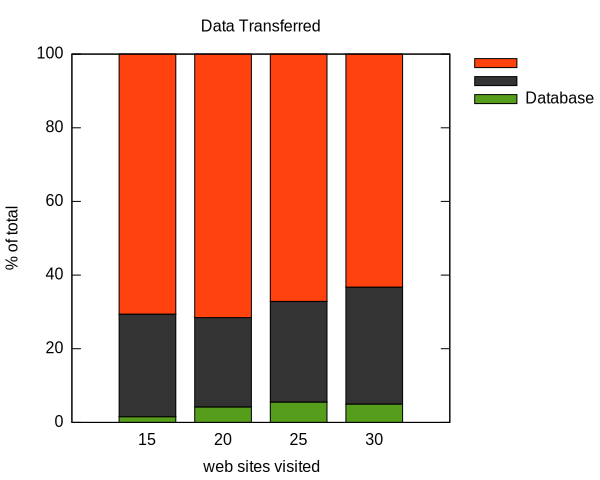
\includegraphics[width=0.75\textwidth, angle=-90]{./img/plots.pdf}
    	\caption{Results of Test 1}
	\label{fig:frontendtest1}
\end{figure}

Table \ref{tbl:times} shows the total time spent and the time spent actually transferring files when retrieving the 15 web page set.

\begin{table}[!h]
		\centering
       \begin{tabular}{| c | c | c | c |}
               \hline
               Phone \# & Total time (s) & Time downloading (s) & Time spent downloading of total time(\%)\\
               \hline
               1 & 251 & 17 & \textbf{6}\\
               \hline
               2 & 303 & 15 & \textbf{4}\\
               \hline
               3 & 241 & 20 & \textbf{8}\\
               \hline
               4 & 254 & 18 & \textbf{7}\\
               \hline
       \end{tabular}
       \caption{Run-times}
       \label{tbl:times}
\end{table}

The results of test two can be seen in Figure \ref{fig:frontendtest2}. The two leftmost bars represent the first repetition of the test and the two right most the second repetition.

\begin{figure}
	\centering
		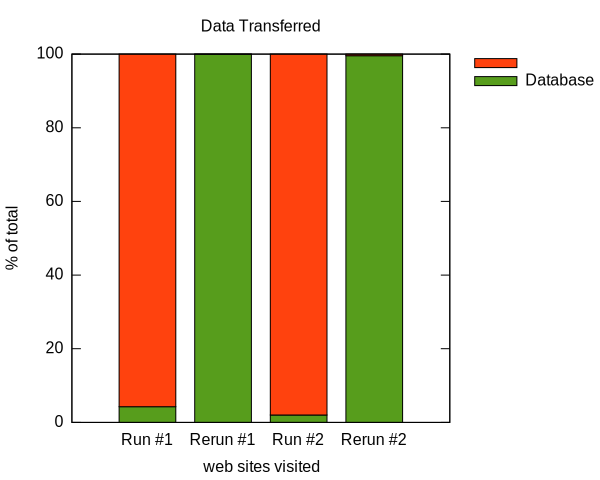
\includegraphics[width=0.75\textwidth, angle=-90]{./img/rerun.pdf}
    	\caption{Results of Test 2}
	\label{fig:frontendtest2}
\end{figure}

The results of the third test can be seen in Figure \ref{fig:frontendtest3}

\begin{figure}
	\centering
		\includegraphics[width=0.75\textwidth, angle=-90]{./img/bt.pdf}
    	\caption{Results of Test 3}
	\label{fig:frontendtest3}
\end{figure}

\subsection{Discussion}

In Figure \ref{fig:frontendtest1}, it can be see that even without precaching, approximately 30\% of the data can be retrieved without accessing the Internet. This corresponds roughly to the 25\% which could be expected if all the resources were unique and successfully cached in the NRS, since in that case only the first phone would retrieve the resource from the Internet. With precaching of popular web pages this percentage could possibly increase even further.

It was observed that if one phone had a jump start on another phone to start retrieving a certain web page, the second phone shortly caught up with the first phone. The two phones then try to retrieve the same resource at the same time which will not be in the cache and both will use the Internet.

In Figure \ref{fig:frontendtest1} it can also be seen that a few percent of resources are retrieved from the database. This is because these resources are linked to several times throughout the web pages. Since the resource is cached in the database the first time, additional requests can use the database.

Figure \ref{fig:frontendtest2} demonstrates that when accessing a web page a second time a small part still has to be retrieved using the Internet. An example of when this can happen is when a web page links to a resource using JavaScript to add a timestamp to the resource's URL. The dynamic nature of this content means that it will not be in any cache when requested. This means there will be a certain amount of resource that will have to be retrieved from the Internet.

In Figure \ref{fig:frontendtest3} it can be seen that the amount of data retrieved using alternate transfer methods are similar whether or not full put is used. This is expected as only the first phone should have to retrieve the data from the Internet. If can also be seen that, as expected, the amount of data retrieved is close to the theoretical 25\% mentioned above.

Table \ref{tbl:times} shows that the retrieval of web pages is very slow, but it can also shows that the actual transfer of files does not contribute to much of the total time. The retrieval is so slow that using this application in a real life situation probably only makes sense if there is no connection at all otherwise. The main culprit behind the long retrieval times seems to be the searches. This is not visible from the logs but when the application is running most of the time is spent searching. A search is done for every web resource and the time quickly adds up. To improve the retrieval times of web pages the search needs to be optimized.

One thing that is not immediately visible but that effects the test result is the fact that NetInfService randomly pauses in the background. If this happens it results in all publishes, gets and searches failing which in turn results in everything being retrieved from the Internet. It is suspected that this is caused by how the Android OS handles applications in the background.
\section{Backend}

The following section describes how the NetInf streaming functionality was evaluated and tested. 

\subsection{Video streaming protocol evaluation}
One of the problems discussed was reducing congestion when broadcasting content. 
This was solved by implementing an alternative way of sending chunked data as seen in 
Section \ref{sec:Chunked data streaming} according to the video streaming draft in 
Appendix \ref{VideoDraft}. In the following section this implementation is referred to
as the \textit{modified streaming}. 
The following tests were conducted:

\begin{itemize}
\item Testing the modified version of NetInf video streaming. 
\item Testing the pure version of NetInf video streaming.
\item Comparison between both implementations of the NetInf Video streaming
\end{itemize}

The testing was done by transferring 500 chunks of bogus data between a number of different NetInf nodes running ERNI. 
All the receiving nodes started the transfer at the same time.
To be able to publish $N$ number of chunks in an easy and fast manner, the \textit{nn\_evaluation} module was implemented.

\subsection{Pure video streaming evaluation setup}
The nodes that were included in the pure version of the streaming were the following:
Central NRS node, one streaming source node that published all 500 NDOs to itself with 
\textit{fullput} set to True, then also published the NDO to the central NRS with 
\textit{fullput} set to False. The central NRS can not have the octets 
because otherwise it would provide all clients with the octects directly, 
hence prevent the network load to be more balanced.

Five client nodes then got each chunk by:
\begin{enumerate}
\item searching NRS for the chunk with chunk number and stream name.
\item getting the NDO metadata and locators from the NRS.
\item fetching NDO with octects from one of the locators.
\item publishing the NDO to itself 
\item adding itself as a locator and publish to the NRS.
\item repeating the procedure for the next chunk.
\end{enumerate}

\subsection{Modified video streaming evaluation setup}
In this setup one node served both as the source and central NRS while there 
were five other client nodes. The source first published the stream NDO to itself, 
then used the content dispatcher to put all the chunks into the storage.
The clients then get the streamed NDO, added themselves as 
locator and published it to the NRS. To retrieve the chunks each client need to:

\begin{enumerate}
\item append the current chunk number to the NDO name.
\item send the request to one of the locators.
\item if status of the response is 404, repeat step 2.
\item store the octects in its storage.
\item increase the chunk number
\end{enumerate}

\subsection{Results} 
The Figure~\ref{fig:eval-stream-modvspure} shows 
that the pure NetInf streaming is faster when it comes to 
transferring all the chunks. 

The CPU load of the central NRS was recorded with the built in system monitor, 
the result of the pure version is in Figure~\ref{fig:eval-stream-pure-cpu} and the modified in Figure~\ref{fig:eval-stream-mod-cpu}. 


\begin{figure}[h!]
	\centering
		\includegraphics[width=0.75\textwidth]{./img/eval-stream-plot-modvspure.png}
    	\caption{Pure streaming vs modified streaming}
	\label{fig:eval-stream-modvspure}
\end{figure}

\begin{figure}[h!]
	\centering
		\includegraphics[width=0.75\textwidth]{./img/eval-stream-pure-cpu.png}
    	\caption{Central NRS CPU usage during pure streaming}
	\label{fig:eval-stream-pure-cpu}
\end{figure}

\begin{figure}[h!]
	\centering
		\includegraphics[width=0.75\textwidth]{./img/eval-stream-mod-cpu.png}
    	\caption{Central NRS CPU usage during modified streaming}
	\label{fig:eval-stream-mod-cpu}
\end{figure}

\subsection{Discussion}
As can be seen in Figure~\ref{fig:eval-stream-modvspure} the transfer of the chunks 
took less time using the pure streaming, this was not unexpected since the modified version has a lot of overhead in this case, 
if it tries to get chunks from another client which does not have them yet, 
this will yield in an 404 response and the client will need to try another source. 
The pure NetInf however will get a hit every time. 

Comparing CPU load in Figure~\ref{fig:eval-stream-pure-cpu} and Figure~\ref{fig:eval-stream-mod-cpu}, 
it shows that even with only five receiving nodes the pure central NRS was under considerably high load,
while the modified versions load was almost not noticeable. The CPU load on the pure NRS is caused by  
the number of database lookups. 

\subsection{Notes on Interoperability}

There are already existing implementations created by SAIL and Ericsson Research 
for the NetInf protocol\citation{netinfproto}. In the beginning of the product 
life-cycle the customer requested the development team to evaluate the interoperability 
of this product with other systems. However as the product evolved the customer requested 
that the interoperability be left to them to evaluate and that this development team 
continue with evaluating the video streaming instead.

Therefore the development team did not evaluate interoperability, but there is confidence
that with minor tweaking of the code (due to differences in the various draft versions of
the NetInf protocol specification) this product and others will become interoperable.

The following list describes the evaluation performed for testing the NetInf NRS application.

\begin{itemize}
\item Evaluation of the search time and get time for the supported databases
\item Measuring the number of requests per frontend phone client
\end{itemize}


\chapter{Conclusions and Future Work}
\label{sec:conclusions}
\section{Conclusions}
The main goal of this project was to develop an application based on the principles of information centric networking using the NetInf protocol. This goal was achieved and the project team was able to build this application using Java and Erlang/OTP. It is a distributed, concurrent and fault tolerant application as per the principles of OTP. The project team had a clear goal in its sight when it started this project and achieved it comfortably in the end. Infact, the team added the functionality to support streaming videos using the application. This functionality was not part of the original plan but because the team achieved all the other major goals well before time, it had the time to add this functionality at the end. 

The client for this project Ericsson Research was also satisfied with the work done by the project team. 

\section{Future Work}

\subsection{Elephant and NetInfService}

\subsubsection{Dynamic Content}

Currently the dynamic content problem is ignored. The browser application uses NetInf search to find NDOs corresponding to web pages. That is, given a traditional web URL we want to map to an NDO. As long as the web content is static the mapping from URL to NDO will be one-to-one. However, if the web content is dynamic the mapping will be one-to-many. If this is the case a search could return several matching NDOs. At a first glance adding the time the page was retrieved as metadata could seem to solve the problem. While this is true for some dynamic web pages, it does not hold in general. For example a web page could be generated differently depending on who or from where it was accessed. Further, a dynamic web page linking to other dynamic resources might be dependant on getting the correct version of the linked resources. In the second case a timestamp could help if all resources belonging together are marked with the same timestamp and not the individual access times.

\subsubsection{Precaching}

If the NetInf network starts without any web content cached there will be a lot of Internet access in the beginning while the content is entering the network. This could be prevented by precaching content in, for example, the NRS. By investigating which web pages are frequently accessed and when they are accessed the NRS could download these in advance. If the search requests always use the NRS this information will be continuously available to the NRS and it could automatically downloaded pages it expects to be accessed when there is bandwidth to spare.

\subsubsection{Search}

The Elephant browser relies heavily on NetInf searches as described in Sections \ref{sec:Elephant Web Browser} and \ref{sec:Elephant}. Currently the time needed to perform a search quickly increases as the number of published NDOs increase. The NRS supports two ways of saving published NDOs either using an Erlang list or a Riak database. Preliminary tests had problems with increasing search times using both these approaches. It is possible the slowdown is caused by the NetInfService or Elephant applications for some reason. Investigation into the reason behind this slowdown is required to improve the performance of the Elephant browser.

\subsubsection{Delete Functionality}

Currently the NetInf delete functionality is not provided by the NetInfService. However, the framework for its implementation is in place so adding this functionality should require relatively little work.

\subsubsection{NetInfService}

NetInfService was implemented as its own Android application which is supposed to run in the background. While this makes it easy to create other applications using the provided functionality there are currently some problems with the application randomly stopping and not resuming until it is brought to the front. The suspected reason is that the Android OS might pause applications in the background to save system resources or stop them when system settings are changed and then restart them when they are brought to the front. If this is an unavoidable problem for Android applications running in the background then NetInfService needs to be changed, perhaps into an Android Service. More investigation is required.

\subsection{Access Control}

Currently any user can publish his content on the NRS. One functionality for the future could be to implement some kind of access control mechanism. Only authorized users would be able to publish on a particular NRS and only a partiular group of users would be able to access the published content. 

\subsection{Interoperability}

Another interesting task for the future could be to test the interoperability between different NetInf implementations. There are different implementations of NetInf in different programming languages. They should be able to communicate with each other if they have been implemented using the same protocol. 

\subsection{Handle large file}

Currently the application built by the project team experiences problems while dealing with files over 10 mega bytes. An improvement to the application could be make it handle larger files.

\subsection{Database and Bluetooth convergence layer}

Other suggestions for future work include testing the application with another database like SQLite or building a bluetooth convergence layer for users to be able to send NetInf messages via bluetooth. 


\chapter{Appendix A: Installation instructions}
\section {Frontend}

In this section we will take a look at how to configure
our environment to run our application on an Android phone. 
This description includes
configuring Eclipse with Android in order to further develop on our 
project. We assume that you already have the Java SDK and Eclipse installed.

For our project we have been working with:
\begin{itemize}
\item Eclipse Indigo Service Release 2
\item Android Version 4.1.2
\end{itemize}

\section{Configuring Eclipse with Android}
In order to configure Eclipse with Android, follow these
instructions:

\href{http://developer.android.com/sdk/installing/installing-adt.html}{Eclipse-Android configuration}
\section{Installing the application}

\section {Backend}
In this section we will see how to install and setup the Netinf NRS and the NetInf Streaming on a server.
This description includes instructions on how to setup the system for both development and normal uses.

\subsection{Dependencies}

In order to run the system properly the following components are required to be installed on the system




\subsection{Script}

For the convenience of end users and developers, there is a packaged install/setup script available after obtaining the backend code.

\textbf{note if the script is not immediately runnable for you please run the following command:}
\begin{verbatim}
chmod a+x netinf_nrs.sh
\end{verbatim}

You can run the script by using the following on a command line terminal

\begin{verbatim}
./netinf_nrs.sh
\end{verbatim}

The script will put you into a menu loop shown below and instructs you to type a number in order to choose an option.Choosing an option will preform the task and then cause the script to exit normally.

\includegraphics[scale=0.5]{./img/Backend_install_script.png}

The following options are available to the user

\begin{itemize}
\item Start Netinf NRS with the default list\\
Assumes you have all the dependencies installed and only starts the netinf nrs with the list database.
\item Start Netinf NRS with riak\\
Will check that riak is running and present in the system and then start the netinf nrs with the Riak database.
If riak is not present then the script will download and install all the required components. 
\item Install and setup riak only\\
Use this option only when you want to download and install riak on your machine. This will not start an NRS.
\item Install and start from scratch\\
This option assumes you have a bare machine and checks that all the dependencies are satisfied. It will auto download and install anything that is required and then start your NetInf NRS with the default list database. 
\end{itemize}


\subsection{Riak Database}

Riak is a database written in Erlang. It is known for being distributed and fault-tolerant. Riak was choosen above other database implementations since it was suggested by the client and the development team had great support available. 

In case there is something wrong with the script process on the target machine please follow the manual installation instructions below.

Install libssl0.9.8 with
\begin {verbatim}
sudo apt-get install libssl0.9.8
\end{verbatim}

Next install the riak database
\begin{verbatim}
wget http://downloads.basho.com.s3-website-us-east-1.amazonaws.com/riak/CURRENT/ubuntu/lucid/riak_1.2.1-1_i386.deb
sudo dpkg -i riak_1.2.1-1_i386.deb
\end{verbatim}

In order for the search to work in the riak system and from the NRS please enable search.
Riak Search is enabled in the app.config (/etc/riak/app.config) file. Simply change the setting to “true” in Riak Search Config section (shown below).

\begin{verbatim}
%% Riak Search Config
{riak_search, [
               %% To enable Search functionality set this 'true'.
               {enabled, false}
              ]},
\end{verbatim}

Then run the in the terminal

\begin{verbatim}
riak restart
\end{verbatim}

Followed by to index the bucket

\begin{verbatim}
search-cmd install netinf_bucket
\end{verbatim}

Lastly, please make sure that the NRS is started with the riak database



\chapter {Appendix B: Maintenance instructions}

\section{Frontend}
\label{sec:Frontend Installation Instructions}
App-B-Maintenance instructions frontend filler
\section{Backend}
The following section describes the maintenance and default settings of the ERNI teams NetInf NRS as well as the NetInf Video Streaming.

\subsection{Default Application Settings}

The NetInf NRS application is controlled using one of two methods, first through the Erlang application src file(netinf\_nrs.app) found in the netinf\_nrs/src directory. The second from the configuration files loaded at run time from the configs directory. 

By default the following settings are used when you do not specify on the Erlang command line which config file to use, please refer to section \ref{Meaning of the config values} to understand what each setting is used for. 

In short, the list database will be attached to the instance of the Erlang NetInf NRS.

\begin{description}
\item[database]
nn\_database\_list
\item[convergence\_layers]
["http"]
\item[ip\_timer]
5000
\item[discovery]
off
\item[nrs\_port]
9999
\item[ct\_port]
8077
\item[client\_port]
8079
\item[list\_timer]
3600
\end{description}

\subsection {Development Environment}

To those wishing to continue the development of the NetInf NRS and the NetInf Video Streaming. The following section details how our development environment was set up. 

Please note that the applications were developed on the Ubutnu 12.04 LTS platform, deviating from this may cause the application to behave in unexpected ways.

The recommended editor used was emacs with the erlang-mode, this editor and mode can be installed using the following commands:

\begin{itemize}
\item sudo apt-get install emacs
\item sudo apt-get install erlang-mode
\end{itemize}

Useful emacs commands include:

\begin{itemize}
\item ALT+X \\
sets up emacs for the meta-command mode. Here you can enter the erlang-mode by typing
ALT+X erlang-mode
\item CTRL+X+S \\
Emacs quick short cut for saving files
\item CTRL+C+K \\
Emacs quick short cut for compiling and saving Erlang files
\item CTRL+X 1-3 \\
Emacs quick short for dividing the windows into 1 whole window, horizontally or vertically.
\end{itemize}

Please note that Emacs has auto-completion for commands when pressing tab. Other useful tips include Erlang-mode skeletons which allow the developer to import comment sections and whole skeletons for generic servers and behaviours.

\subsection {Code and folder structure}

The NetInf NRS and the NetInf Video Streaming application are organized in the following way

\begin{description}
\item [netinf\_nrs]
The main folder which holds the code, config, make and the important files for the application.
\item [configs]
The folder which contains all the configuration files for the NetInf NRS application. Please place all the new configuration files here. 
\item [curludp]
This folder contains a text file which the is read from the udp\_test.sh. It has no other uses.
\item [deps]
This folder is created automatically from running the rebar( or the script, which invokes makes and eventually rebar). It contains all the dependency code required for libraries that were used in the NetInf NRS application. 
\item [doc]
This folder is created automatically from running the rebar doc command (see section fix ref here below). Use the index.html file to get to the first page of the documentation. Please note that this is normally not present unless you run the doc command.
\item [ebin]
This folder contains all the compiled Erlang beam files, this is where the Erlang virtual machine will look for the compiled code modules.
\item [files]
This folder contains all the stored binary content(NDO cache). The NetInf NRS will look here and determine if it has the content or not if the NRS recieves a get message, alternatively if the NRS receives a publish message with binary octets it will save it here. This folder is required for the NRS to start properly.
\item [logs]
This folder contains all the logging files, it also contains a folder named old. The logger service in the NRS will create a text file with information about the NRS and current activities here up to a default size of 10MB (may be changed in the nrs\_logger.erl file in the src directory). This folder is required for the NRS to start properly.
\item [resources]
This folder contains all the resources for the HTML client interface for the NetInf NRS video streaming.
\item [src]
This folder contains all the source code for both the NetInf NRS and the video streaming.
\end{description}

Please note that inside the main netinf\_nrs folder are several files consisting of a Makefile, rebar.config file, udp\_test.sh -udp testing script, readme and the netinf\_nrs startup/install script. 

\begin{description}
\item[Makefile]
This is the make file with several targets shown below. It is primarily used for compiling the NetInf Nrs project and invoked now by the main netinf\_nrs script. 
\begin{itemize}
\item all \\
Creates the required folders for the environment, compiles both erlang source code and the json c++ and finally runs eunit but this does not start the NRS.
\item all\_no\_test \\
Same as the above, however it does not invoke the eunit tests.
\item eunit \\
Runs the eunit tests using the rebar and skips all the dependency tests(only tests NetInf NRS).
\item integration\_test \\
compiles the Erlang source code and the dependencies if need be and then runs only the integration\_test code.
\item integration\_test\_riak \\
Same as the above but will attach the riak database to the Erlang NetInf NRS instance and run the integration\_test code on that.
\item makec \\
Compiles only the c++ json dependency code in the deps folder. 
\item set\_env\_folders \\
First removes the following  required folders: logs and files, then re-creates them.
\item compile \\
First tests if the deps folder already exists then compiles the dependencies, otherwise it will get all the required dependencies and then compile them.
\item compile\_deps \\
cleans the deps folder then downloads all the dependencies again and compiles them.
\item start\_script\_riak \\
Runs the steps in the all\_no\_test target then starts the NetInf NRS with the riak database attached.
\item start\_script \\
Runs the steps in the all\_no\_test target then starts the NetInf NRS with the default list database attached.
\item clean \\
removes the environment folders (logs and files) and removes the ebin compiled folders as well as the crash dump if the Erlang virtual machine crashed.
\end{itemize}
\item[rebar.config]
This file defines all the settings for rebar in this particular project. The dependencies as well as options for eunit and various plugins to rebar can be configured.
\item[udp\_test.sh]
This file is a script for testing the UDP convergence layer. Please note it is best tested with the discovery off in the config file. You must have at least two different computers to run these tests. All instructions are in the script. 
\item[netinf\_nrs.sh]
This file is the main setup/install and run script. Please use this to install all the required components on the machine to ensure maximum compatibility. More details about this script can been seen in \ref{Appendix-A/App-A-Installation_instructions_backend.tex}
\end{description}

\subsection {NetInf NRS modules}

The main code modules are located in the /src directory of the main folder. Each file has comments inside which can be generated into documentation please see subsection \ref{Generating documentation}

\begin{description}
\item[Erlang-application file]
Erlang applications require a definition file in order for the Erlang virtual machine to be able to understand which modules need to be preloaded and what configurations if any need to be supplied to the application
\begin{itemize}
\item netinf\_nrs.app.src - this file gets read by the Erlang virtual machine at compile time. Developers can set various options for the default settings in the "env" section of the file.
\end{itemize}
\item[Supervisors]
Erlang uses supervisors to organize which process must stay alive for a application to function as intended, below is a brief description of all the supervisors required in the NetInf NRS application
\begin{itemize}
\item nn\_sup - This is the main supervisor which starts the \ldots
\item nn\_sub\_supervisor - This is the sub supervisor. It is responsible for starting \ldots
\item nn\_client\_supervisor - This is the client supervisor. It is responsible for starting \ldots
\item nn\_msgid\_sup - This is the message id supervisor. It is responsible for starting \ldots
\end{itemize}
\item[Convergence-Layers]
As stated in section \textbf{insert section numbers here} the application was designed to be modular, the idea of convergence-layers allowed the application to group three distinct modules together to create the convergence-layer in erlang.
\begin{itemize}
\item nn\_http\_handler 
\item nn\_http\_forwarder
\item nn\_http\_formatting
\item nn\_udp\_handler
\item nn\_udp\_forwarder
\item nn\_udp\_formatting
\item nn\_message\_handler
\item nn\_message\_formatting
\end{itemize}
\item[Database behaviour \& Storage interface]
This application contains a custom behaviour to allow developers to quickly create wrappers for databases as well as functionality to change the database at run-time. The following modules are involved:
\begin {itemize}
\item nn\_database - This is the custom behaviour implemented for creating database wrappers. Each new database wrapper must include this file in the header. Erlang will then tell you if you are missing some functions when you implement a new database wrapper. See section  PNP Database Wrapper {fix ref here} for more information.
\item nn\_storage - This is the interface between the database wrapper and the content caching. This module is responsible for facilitating requests from the event\_handler.
\end{itemize}
\item[Databases]
The NetInf NRS application has support for various plug and play database wrappers. As long as the developer adheres to the required input and output of the database behaviour this application can be extended to work with any database. 
\begin{itemize}
\item nn\_database\_list - This module implements the callback functions defined in the nn\_database. It is also a quick database consisting of a persistant Erlang list data structure. The module also has a timer which causes the list structure to be saved to disk every hour. This can be controlled in the configs/list.config file under the appropriate variable.
\item nn\_database\_riak - This module implements the callback functions defined in nn\_database, it is a wrapper for talking to a riak process (riak is a standalone database).
\end{itemize}
\item[Content-Caching]
The NetInf NRS also includes a method of caching binary objects sent into the system via NetInf messages, the following are the two modules involved in this functionality.
\begin {itemize}
\item nn\_content\_handler - This module
\item nn\_hash\_validation - This module validates the hash of the NDO coming in to the one that is currently stored in the files folder. Please note that the files folder must be present in the system otherwise the application will crash. 
\end{itemize}
\item[NetInf Video Streaming]
The NetInf NRS application supports a video streaming protocol on top of the existing application. The main files used in this protocol are described here, please note that the video streaming also relies on the resources folder as well to provide the http client interface to the user. 

\begin{itemize}
\item nn\_subscribe
\item nn\_stream\_handler
\item nn\_stats
\item nn\_ct\_handler
\item nn\_http\_client\_handler
\item nn\_http\_ct\_handler
\end{itemize}

\item[Logger]
The NetInf NRS application supports a file based logging method, which creates a file named log.txt in the logs folder. The logger comes with 3 levels verbose, warning and error. Developers can choose which level to log at in the configuration file. By default the log file sizes are set to 10MB and then the log file gets moved to the old/ folder. You can increase this in the nn\_logger module under the macro LOG\_FILE\_SIZE.
\begin{itemize}
\item nn\_logger
\item nn\_logger\_server
\item nn\_log\_handler
\end{itemize}
\item [Utility \& Misc]
The following modules are used to expose a variety of functions through out the system.
\begin{itemize}
\item nn\_util - This module contains many useful functions that were being used in multiple modules. It is recommended to read through the functions here as a function may have already been created and exposed to the developers.
\item nn\_merging - This module contains all the functions for merging metadata in the NetInf NRS messages.It uses the json library extensively.
\item nn\_msgide
\item nn\_msgids
\item nn\_msgid\_store
\end {itemize}
\item [Integration test]
The NetInf NRS application required a test in order to check if all the modules were working as intended using the black box testing technique. 
\begin{itemize}
\item nn\_integration\_test - This module contains the black box level tests for the entire NetInf NRS system.
\end{itemize}


\end{description}

The majority of the above modules have unit tests for them in the same folder, they are denoted with the same starting name but also have the \_test as well. 

netinf\_nrs - holds the main code for starting and stopping the application along with all the required dependencies(Ranch, Crypto, Cowboy).

nn\_app - Starting point of the nn application. Initiates an http listener and starts the main supervisor and reads all the configuration settings from the config files or the env from the netinf\_nrs.app.src file.

nn\_event\_handler -This module

nn\_proto - This module contains the internal representation of a NetInf message based on the draft. It also contains functions to get and set the messages. It is used in many modules and it is part of the core NetInf NRS architecture.

nn\_discovery\_service
nn\_discovery\_client


\subsection{Generating documentation}

Code documentation for the application can be generated by running the following commands in the terminal when in the main netinf\_nrs folder.

\begin{verbatim}
rebar doc skip_deps=true
\end{verbatim}

This will create a new folder doc/ in the main netinf\_nrs folder. The documentation should be read from the file named index.html




\chapter {Appendix C: NetInf Video Streaming Draft}
\section {NetInf Video Streaming Protocol}\label{VideoDraft}

\subsection{Introduction}

The purpose of this draft is to outline a design and protocol specification for enabling of streaming and chunking data within the current and existing netinf architecture.

\subsubsection{Proposed method of retrieving chunked NDOs}

The stream source will PUBLISH an NDO containing the filename as content. The object is marked as a stream in the metadata. It also contains a locator to the stream source.

In order to access the stream, a receiver will first perform a NetInf-GET on the above filename object in order to retrieve the locator. 

In the next step the client can get the chunks. By replacing the hash algorithm in the NDO-name with \_demo\_ and sending a NetInf-Get to the source, the stream provider will return the octets of the most recent chunk and the chunk number in the metadata. This implies that the regular hash validation has been disabled.

For further chunks, the receiver will increment the chunk number and append it to the locator.
\begin{verbatim}
If a stream is published with the name
 ni:///sha-256;WkOCMB2aEQHrARjTldfhRE5OgZkZmCHzokcoVMnfp2Y

You can get latest chunk by fetching
 ni:///demo;WkOCMB2aEQHrARjTldfhRE5OgZkZmCHzokcoVMnfp2Y

To get first chunk, append a 1 to the end of the hash
 ni:///demo;WkOCMB2aEQHrARjTldfhRE5OgZkZmCHzokcoVMnfp2Y1

To get the 32th chunk, append 32 to the end of the hash
 ni:///demo;WkOCMB2aEQHrARjTldfhRE5OgZkZmCHzokcoVMnfp2Y32
\end{verbatim}
 
If the receiver also acts as a cache, it will send a PUBLISH with the filename object and a locator pointing to itself to the NRS.
\\

\includegraphics[scale=0.5]{./img/sequence_diagram_streaming.png}

\subsubsection{Testing criteria} 

For a simple test setup, in addition to the NetInf node, a receiving and a publishing client is required. A more sophisticated test could involve multiple receivers, to demonstrate the caching.

A use case for testing is one where the source of the content is a pre-encoded video file of a particular size.

The example below assumes a video file of the size 700 megabytes.

A client (Publisher) will have a default chunk size which is used to chunk up the source file. For this example, 1 megabyte chunks will be used.

Thus, it can be calculated that the publisher will create 700 chunks of the size 1 megabyte, numbered 1-700.

A second client (receiver) knowing the name of the video file will then send a Get request to the NetInf node (to keep things simple, it is assumed that the object's name is already known).

The client will now start generating consecutive GET requests with the sequence numbers constantly increasing and expect to receive the appropriate chunk.

As well as  poll the NRS for new locators, to get better load balance between nodes contributing to the stream.

This process occures until the GET requests generate a 404 because the unique sequence number has increased past the last published chunk number.

\subsubsection{Extra notes}

Chunk size is going to be a configurable option in the publishing client.

\chapter {Appendix D: License}
\input{Appendix-D/license.tex}
\bibliography{references}
\bibliographystyle{plain}


\end{document}
